\section{Introducci\'on}

\begin{frame}
 \frametitle{Resumen}
%  \framesubtitle{}
 \begin{exampleblock}{
  \begin{center}
	\textbf{Medici\'on del flujo de neutrinos c\'osmicos ultra energ\'eticos mediante detectores de superficie}
  \end{center}
  }
  \begin{enumerate}\setlength\itemsep{3mm}
   \item Introducci\'on
   \item Detecci\'on con el observatorio Pierre Auger
   \item Detecci\'on con un arreglo de antenas de radio
  \end{enumerate}

 \end{exampleblock}
\end{frame}

\begin{frame}
 \frametitle{?`Por qu\'e astrof\'isica con neutrinos?}
 \begin{textblock}{15}(0.5,2)
  \begin{block}{Mensajeros de alta energ\'ia}
   \begin{itemize}\setlength\itemsep{2mm}
    \item {\color<2>{OrangeRed}\textbf<2>{Protones}}
    \item {\color<3>{OrangeRed}\textbf<3>{Fotones}}
    \item {\color<4->{OrangeRed}\textbf<4->{Neutrinos}}
   \end{itemize}
  \end{block}
 \end{textblock}
 \begin{textblock}{7.5}(0.5,7.5)
  \begin{block}{Cualidades deseadas}
   \begin{itemize}\setlength\itemsep{3mm}
    \item {\color<2->{Green} Escapan de la zona de aceleraci\'on}
    \item {\color<3,4->{Green}\color<2>{Red} No se deflectan con campos magn\'eticos.}
    \item {\color<4->{Green}\color<2,3>{Red} No pierden energ\'ia en el trayecto}
    \item {\color<2,3>{Green}\color<4->{Red} Es f\'acil detectarlos}
   \end{itemize}
  \end{block}
 \end{textblock}
 
 \begin{textblock}{7}(8.5,7.3)
   \begin{overprint}
    \onslide<1>\vspace*{3.5mm}\centerline{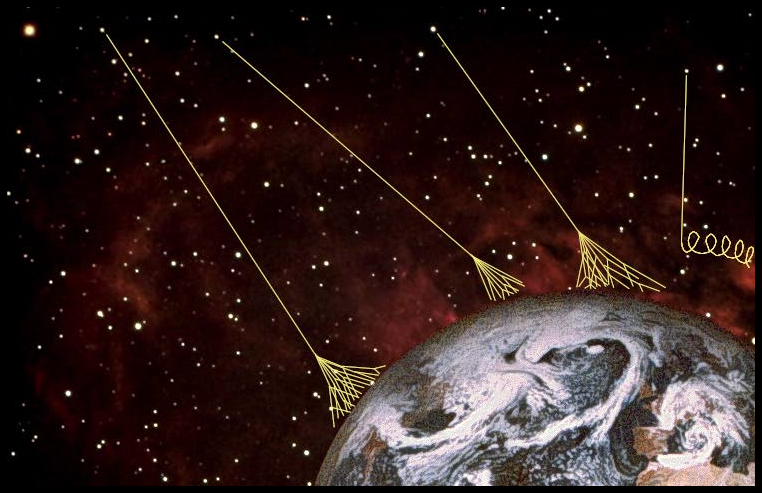
\includegraphics[width=\textwidth]{fig/motivacion/out}}
    \onslide<2>\centerline{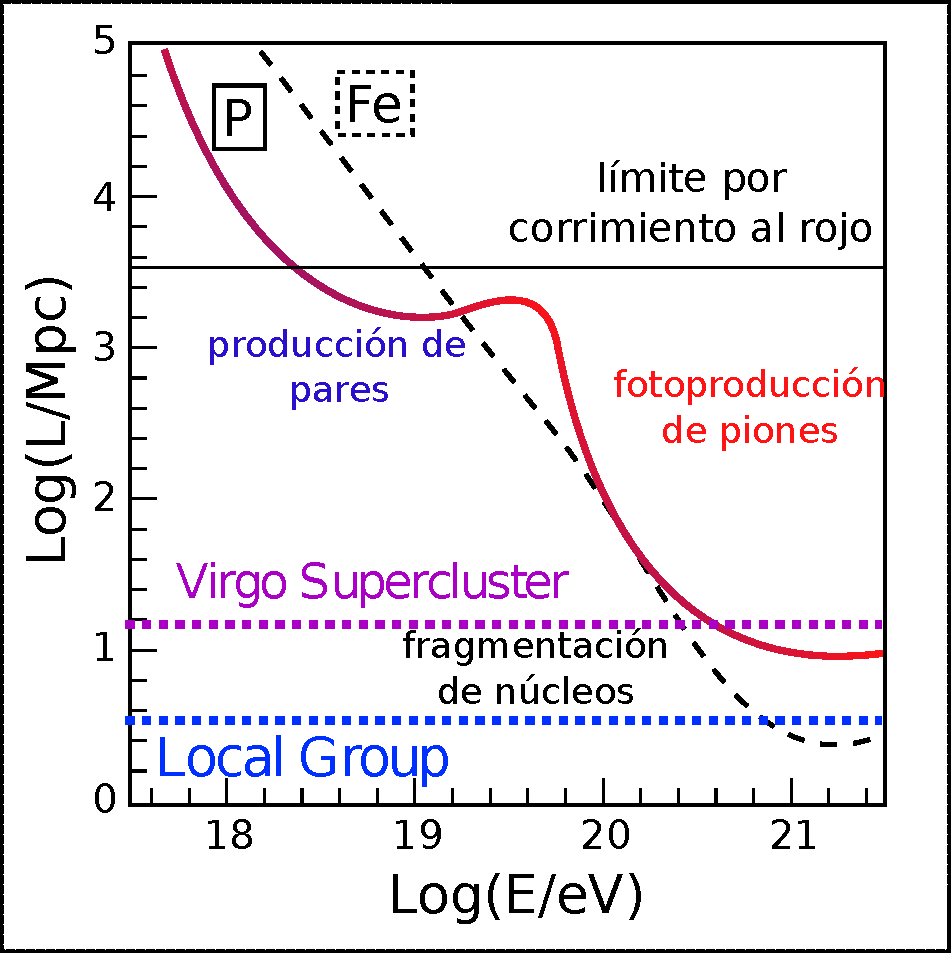
\includegraphics[height=0.75\textwidth]{fig/motivacion/proton}}
    \onslide<3>\centerline{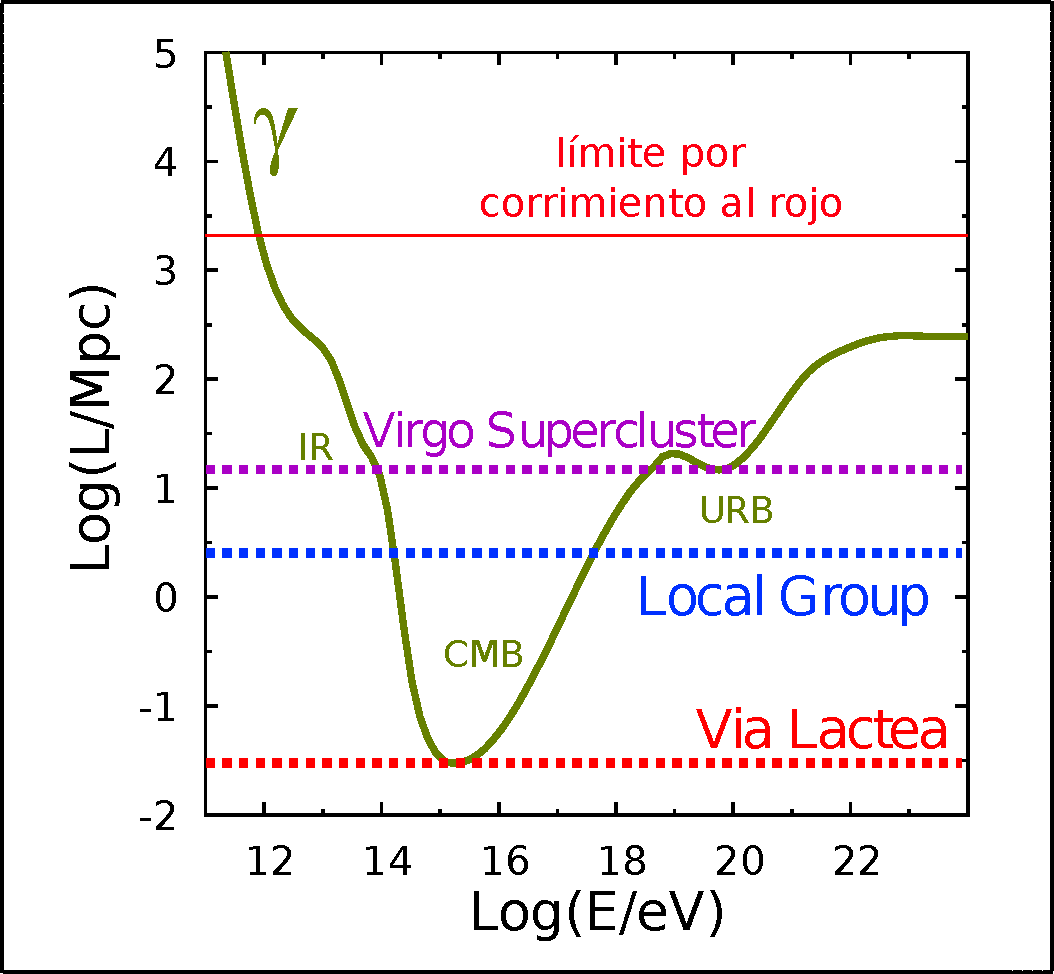
\includegraphics[height=0.75\textwidth]{fig/motivacion/photon}}
    \onslide<4> 
		\vspace*{1cm}
		\begin{block}{}
		\centering 
		\textbf{El desaf\'io consiste en detectarlos!}
		\end{block}
		\vfill
		\begin{alertblock}{Soluci\'on}<5>
		\centering 
		\textbf{Detectores gigantes}
		\end{alertblock}
		\vfill
	\onslide<5>
		\vspace*{1cm}
		\begin{block}{}
		\centering 
		\textbf{El desaf\'io consiste en detectarlos!}
		\end{block}
		\begin{alertblock}{Soluci\'on}
		\centering 
		\textbf{Detectores gigantes}
		\end{alertblock}
   \end{overprint}
 \end{textblock}
\end{frame}

\begin{frame}
 \frametitle{De donde vienen?}
 \begin{alertblock}{}
  \centering
  $\bm{\pi\rightarrow\mu+\nu_\mu\rightarrow e + \nu_e + \nu_\mu}$
 \end{alertblock}

 \begin{block}{Producci\'on en las fuentes (AGN o GRB)}
  \begin{itemize}
   \item Producci\'on via:
   \begin{displaymath}
    \begin{array}{l}
		p + p \rightarrow \pi`s + X \\
		p + \gamma \rightarrow \Delta^{+} \rightarrow p +\pi^{0}\,\,{\rm \acute{o}}\,\, n +\pi^{+} \\
        {\rm otras\,\, resonancias..}
	\end{array}
   \end{displaymath}
  \end{itemize}
 \end{block}
 \vfill
 \begin{center}
  \pgfimage[width=0.65\textwidth]{fig/motivacion/AGN_GRB_nufluxes}
 \end{center}
 \vfill
\end{frame}

\begin{frame}
 \frametitle{De donde vienen?}
 \begin{alertblock}{}
  \centering
  $\bm{\pi\rightarrow\mu+\nu_\mu\rightarrow e + \nu_e + \nu_\mu}$
 \end{alertblock}
 \begin{block}{Cosmog\'enicos o GZK}
  \begin{itemize}
   \item Producci\'on via:
   \begin{displaymath}
    \begin{array}{l}
		p + \gamma_{CMB} \rightarrow \Delta^{+} \rightarrow p +\pi^{0}\,\,{\rm \acute{o}}\,\, n +\pi^{+} \\
        {\rm otras\,\, resonancias..}
	\end{array}
   \end{displaymath}
  \end{itemize}
 \end{block}
 \vfill
 \begin{center}
  \pgfimage[width=0.65\textwidth]{fig/motivacion/gzk_fluxes}
 \end{center}
 \vfill
\end{frame}

\begin{frame}
 \frametitle{Situaci\'on experimental}
 \begin{textblock}{8}(0.5,2.5)
  \pgfimage[width=\textwidth]{fig/motivacion/1510-02050_multimessenger_noAuger}
 \end{textblock}
 \begin{textblock}{6}(9.3,3.5)
  \begin{exampleblock}{Neutrinos medidos por IceCube}
   \begin{itemize}
    \item Flujo aproximado $E^{-2}$
    \item Compatible con protones convertidos en la fuente
   \end{itemize}
  \end{exampleblock}
 \end{textblock}

 \begin{textblock}{8}(7.5,8.7)
 \visible<2>{
  \pgfimage[width=\textwidth]{fig/motivacion/spectrum_withGZK_2015}}
 \end{textblock}
 
 \begin{textblock}{6}(0.5,10.4)
  \begin{alertblock}{Flujo medido por Auger}<2>
   \begin{itemize}
    \item Supresi\'on por encima de $10^{19.5}{\rm\ eV}$
    \item Neutrinos GZK
   \end{itemize}
  \end{alertblock}
 \end{textblock}
\end{frame}

\begin{frame}{Astronom\'ia de neutrinos: experimentos gigantes}
  \begin{center}
    \begin{textblock}{15}(0.5,2.5)
%     \begin{block}{}
      \begin{center}
      \scriptsize\renewcommand{\arraystretch}{1.2}
	\begin{tabular}{llccll} 
      \hline \noalign{\smallskip}
	Experimento      &$E_{\rm min}$  &$E_{\rm max}$       &Ubicaci\'on             &Principio        &Per\'iodo \\
	                 &[eV]           &[eV]                &                        & de detecci\'on                & \\
      \hline \noalign{\smallskip}
      \multicolumn{1}{>{\columncolor{red!50}}l}{ANTARES} &\multicolumn{1}{>{\columncolor{red!50}}l}{$10^{13.5}$}    &\multicolumn{1}{>{\columncolor{red!50}}l}{$10^{15.5}$}   &\multicolumn{1}{>{\columncolor{red!50}}l}{Mar Mediterraneo}    &\multicolumn{1}{>{\columncolor{red!50}}l}{Cherenkov en agua}  &\multicolumn{1}{>{\columncolor{red!50}}l}{2008-} \\
      
      \multicolumn{1}{>{\columncolor{red!50}}l}{Baikal}  &\multicolumn{1}{>{\columncolor{red!50}}l}{$10^{13.5}$}    &\multicolumn{1}{>{\columncolor{red!50}}l}{$10^{16}$}     &\multicolumn{1}{>{\columncolor{red!50}}l}{Siberia} &\multicolumn{1}{>{\columncolor{red!50}}l}{Cherenkov en agua}  &\multicolumn{1}{>{\columncolor{red!50}}l}{1993-}  \\
      
      \multicolumn{1}{>{\columncolor{red!50}}l}{AMANDA}  &\multicolumn{1}{>{\columncolor{red!50}}l}{$10^{13.5}$}    &\multicolumn{1}{>{\columncolor{red!50}}l}{$10^{17.0}$}   &\multicolumn{1}{>{\columncolor{red!50}}l}{Polo sur}           &\multicolumn{1}{>{\columncolor{red!50}}l}{Cherenkov en hielo}    &\multicolumn{1}{>{\columncolor{red!50}}l}{1996-2005} \\
      
      \multicolumn{1}{>{\columncolor{orange!50}}l}{IceCube} &\multicolumn{1}{>{\columncolor{orange!50}}l}{$10^{13.5}$}    &\multicolumn{1}{>{\columncolor{orange!50}}l}{$10^{19}$}     &\multicolumn{1}{>{\columncolor{orange!50}}l}{Polo sur}           &\multicolumn{1}{>{\columncolor{orange!50}}l}{Cherenkov en hielo}    &\multicolumn{1}{>{\columncolor{orange!50}}l}{2006-} \\
      
      \multicolumn{1}{>{\columncolor{yellow!50}}l}{RICE }   &\multicolumn{1}{>{\columncolor{yellow!50}}l}{$10^{17}$}      &\multicolumn{1}{>{\columncolor{yellow!50}}l}{$10^{20}$}     &\multicolumn{1}{>{\columncolor{yellow!50}}l}{Polo sur}           &\multicolumn{1}{>{\columncolor{yellow!50}}l}{Radio en hielo}        &\multicolumn{1}{>{\columncolor{yellow!50}}l}{1999-2005}  \\
      
      \multicolumn{1}{>{\columncolor{yellow!50}}l}{{\bf AUGER}} &\multicolumn{1}{>{\columncolor{yellow!50}}l}{{\boldmath $10^{16.5}$}}      &\multicolumn{1}{>{\columncolor{yellow!50}}l}{\boldmath $10^{20}$}    &\multicolumn{1}{>{\columncolor{yellow!50}}l}{Argentina}            &\multicolumn{1}{>{\columncolor{yellow!50}}l}{{\bf Lluvias atmosf\'ericas}}              &\multicolumn{1}{>{\columncolor{yellow!50}}l}{2004-}\\
      
      \multicolumn{1}{>{\columncolor{yellow!50}}l}{{\bf GRAND}} &\multicolumn{1}{>{\columncolor{yellow!50}}l}{{\boldmath $10^{16.5}$}}      &\multicolumn{1}{>{\columncolor{yellow!50}}l}{\boldmath $10^{20}$}    &\multicolumn{1}{>{\columncolor{yellow!50}}l}{China}            &\multicolumn{1}{>{\columncolor{yellow!50}}l}{{\bf SD radio}}              &\multicolumn{1}{>{\columncolor{yellow!50}}l}{R\&D}\\
      
      \multicolumn{1}{>{\columncolor{yellow!50}}l}{ARA }    &\multicolumn{1}{>{\columncolor{yellow!50}}l}{$10^{16}$}      &\multicolumn{1}{>{\columncolor{yellow!50}}l}{$10^{19}$}     &\multicolumn{1}{>{\columncolor{yellow!50}}l}{Polo sur}           &\multicolumn{1}{>{\columncolor{yellow!50}}l}{Radio en hielo}        &\multicolumn{1}{>{\columncolor{yellow!50}}l}{R\&D}       \\
      
      \multicolumn{1}{>{\columncolor{yellow!50}}l}{ARIANA } &\multicolumn{1}{>{\columncolor{yellow!50}}l}{$10^{17.5}$}    &\multicolumn{1}{>{\columncolor{yellow!50}}l}{$10^{20}$}     &\multicolumn{1}{>{\columncolor{yellow!50}}l}{Ant\'artida}            &\multicolumn{1}{>{\columncolor{yellow!50}}l}{Radio en hielo}        &\multicolumn{1}{>{\columncolor{yellow!50}}l}{R\&D}       \\
      
      \multicolumn{1}{>{\columncolor{yellow!50}}l}{ANITA}   &\multicolumn{1}{>{\columncolor{yellow!50}}l}{$10^{18}$}      &\multicolumn{1}{>{\columncolor{yellow!50}}l}{$10^{23}$}     &\multicolumn{1}{>{\columncolor{yellow!50}}l}{Ant\'artida}            &\multicolumn{1}{>{\columncolor{yellow!50}}l}{Radio en hielo}        &\multicolumn{1}{>{\columncolor{yellow!50}}l}{2007-} \\
      
      \multicolumn{1}{>{\columncolor{blue!50}}l}{GLUE }   &\multicolumn{1}{>{\columncolor{blue!50}}l}{$10^{20}$}      &\multicolumn{1}{>{\columncolor{blue!50}}l}{$10^{23}$}     &\multicolumn{1}{>{\columncolor{blue!50}}l}{California}           &\multicolumn{1}{>{\columncolor{blue!50}}l}{Radio en la Luna}       &\multicolumn{1}{>{\columncolor{blue!50}}l}{1999-2003} \\
      
      \multicolumn{1}{>{\columncolor{blue!50}}l}{LUNASKA} &\multicolumn{1}{>{\columncolor{blue!50}}l}{$10^{21}$}      &\multicolumn{1}{>{\columncolor{blue!50}}l}{$10^{23}$}     &\multicolumn{1}{>{\columncolor{blue!50}}l}{Australia}            &\multicolumn{1}{>{\columncolor{blue!50}}l}{Radio en la Luna}       &\multicolumn{1}{>{\columncolor{blue!50}}l}{2008-} \\
      
      \multicolumn{1}{>{\columncolor{blue!50}}l}{FORTE}   &\multicolumn{1}{>{\columncolor{blue!50}}l}{$10^{22}$}      &\multicolumn{1}{>{\columncolor{blue!50}}l}{$10^{25}$}     &\multicolumn{1}{>{\columncolor{blue!50}}l}{Sat\'elite}            &\multicolumn{1}{>{\columncolor{blue!50}}l}{Radio en la Luna}        &\multicolumn{1}{>{\columncolor{blue!50}}l}{1997-2001} \\
      
      \hline
	\end{tabular}
      \end{center}
%     \end{block}
    \end{textblock}
  \end{center}

%   \setbeamercolor{block body}{bg=black!60!white}
  \begin{textblock}{8}(0.5,12)
  \small
  \begin{itemize}
  \item \colorbox{red!50}{Producci\'on en las fuentes}
  \item \colorbox{yellow!50}{Neutrinos GZK}
  \item \colorbox{blue!50}{Neutrinos no convencionales}
  \end{itemize}
  \end{textblock}

\end{frame}
